\documentclass[../main.tex]{subfiles}
\graphicspath{{./images/}}
%%%%%%%%%%%%%%%%%%%%%%%%%%%%%%%%%%%%%%%%%%%%%%%%%%%%%%%%%%%%%%%%%

\begin{document}


\section{Combining the 2D and 3D approaches} \label{sec:2D_3D_approaches}
This section is devoted to the combination of some of the methods explained in sections \ref{sec:2D_approach} and \ref{sec:3D_approach}. The aim is to try achieve good detection results by leveraging the strengths of each approach in a modular manner. 

\subsection{The recognition pipeline}
It is of specific importance the way in which the two approaches have been glued together. It has been done by dumping information into a `.json' dictionary, written to and read from when switching from the 2D approach to the 3D approach. All segmentation methods explained under section \ref{sec:3D_approach}, sections \ref{sec:sac_segmentation}, \ref{sec:euclidean_segmentation} and \ref{sec:regiongrowing_segmentation} to be specific, display in a visualization window their results on the input point cloud. With the visualization window opened, a key `s' callback is set. When pressed, the program computes bounding boxes for the clusters, and stores them in said `.json' file. Although simpler, its format has some similarities to the one used for the GUI explained in section \ref{sec:GUI}. It is detailed below:
\begin{itemize}
    \item \texttt{annotation}: a list of arbitrary length, containing
    \begin{itemize}
        \item \texttt{bbox}: bounding that encloses the points, in the form of \\$[x_{min}, y_{min}, z_{min}, height, width, depth]$.
        \item \texttt{category\_id}: integer that designates a label. Left to -1 (unknown) by default.
        \item \texttt{npoints}: number of points inside the bounding box.
    \end{itemize}
    \item \texttt{info}
    \begin{itemize}
        \item \texttt{contributor}: name of the person or institution to whom belongs the point cloud and label file.
        \item \texttt{description}: description of the point cloud, if necessary.
        \item \texttt{year}: year in which the labels file is created.
    \end{itemize}
    \item \texttt{image}
    \begin{itemize}
        \item \texttt{file\_name}: file name of the point cloud that corresponds to this label.
        \item \texttt{height}: height of the point cloud as defined by the PCL framework, almost always left to 1.
        \item \texttt{width}: width of the point cloud, almost always is the total number of points in the cloud.
        \item \texttt{npoints}: total number of points were height not to be 1.
    \end{itemize}
\end{itemize}

As mentioned, upon pressing `s', the clusters created by the segmentation methods generate `.json' dictionaries of the type above. The idea is to have a broad segmentation to the input cloud that is \emph{good enough} and then be picked by another 2D computer vision algorithm able to discern which clusters are the objects that are being sought after and which others are not. The bounding boxes in the `.json', however, are in 3D and with reference to the cloud's coordinate frame. Hence, bounding boxes' $[x_{min}, y_{min}, z_{min}, height, width, depth]$  coordinates need to be projected from the 3D point cloud to a position in the plane. In section \ref{sec:using_realsense_sdk} it was mentioned that for every capture taken 3 thing would happen: (1) the point cloud is saved as `.pcd'; (2) the colorized depth image is saved as `.png' and (3) the camera intrinsic values are stored in `.json' format.  It's these intrinsic camera values that need to be leveraged to project the 3D bounding boxes to the image. The same Intel RealSense SDK already provides a function to do that, and accounts for the distortion effects that could have been used when capturing the samples. Here is presented the equation it uses behind the scenes for when there is no distortion (which is the case for this project):

\begin{align} \label{eq:project_IntelSDK}
    x_{2D} = x_{3D} / z_{3D} \cdot fx + ppx;\\ \nonumber
    y_{2D} = y_{3D} / z_{3D} \cdot fy + ppy; \nonumber 
\end{align}

Equation \ref{eq:project_IntelSDK} is used for the 3D bounding box's minimum corners $[x_{min}, y_{min}, z_{min}]$ and maximum corners $[x_{min} + height, y_{min} + width, z_{min} + depth]$ and returns the 2D bounding box positions. These are used to crop the image, and feeding each crop (after resizing that is) to a computer vision algorithm that will try to discern to which class does said crop belong to. Its decision is then inserted into the \texttt{category\_id} entry of the `.json' dictionary, indicating that all points inside its bounding box belong to that new class. This pipeline is visually presented in figure \ref{fig:2D_3D_pipeline}.

\begin{figure}[H]
    \centering
    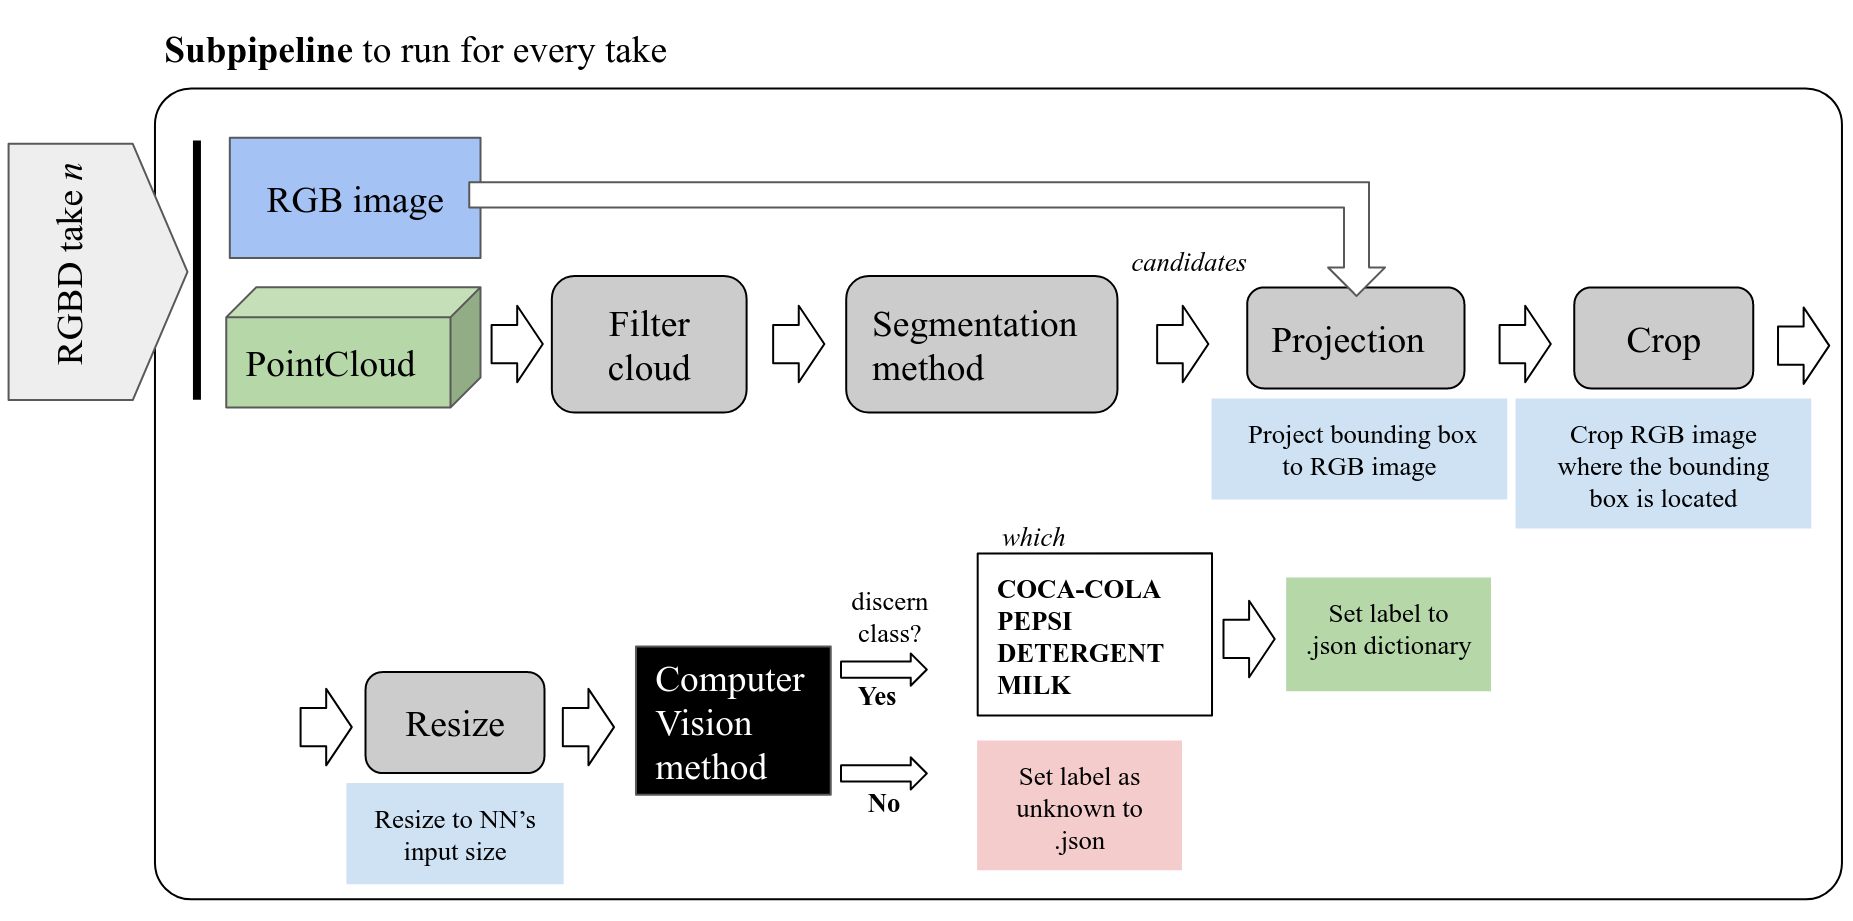
\includegraphics[width=1\linewidth]{images/2D_3D_pipeline.png}
    \caption{The pipeline for joint 3D and 2D detection methods. Note that the blocs `Segmentation method' and `Computer Vision method' are left ambiguous on purpose. They can be any method from the ones covered on this thesis.}
    \label{fig:2D_3D_pipeline}
\end{figure}

For the tests, the algorithm chosen to segment the cloud is only region growing segmentation. It produces many clusters, most of them noise, but segments in coherent pieces the objects in the testbench. It is combined with minimum and maximum cluster points to alleviate the noise. This can be seen in figure \ref{fig:annotated_3Dbboxes_allUnknown}, where the clusters are drawn along with their enclosing bounding boxes. Since they are all marked as unknown, they appear in red. The computer vision algorithms used to disambiguate the clusters are a subset of the ones presented. The results are presented in the subsections below.

\begin{figure}[H]
    \centering
    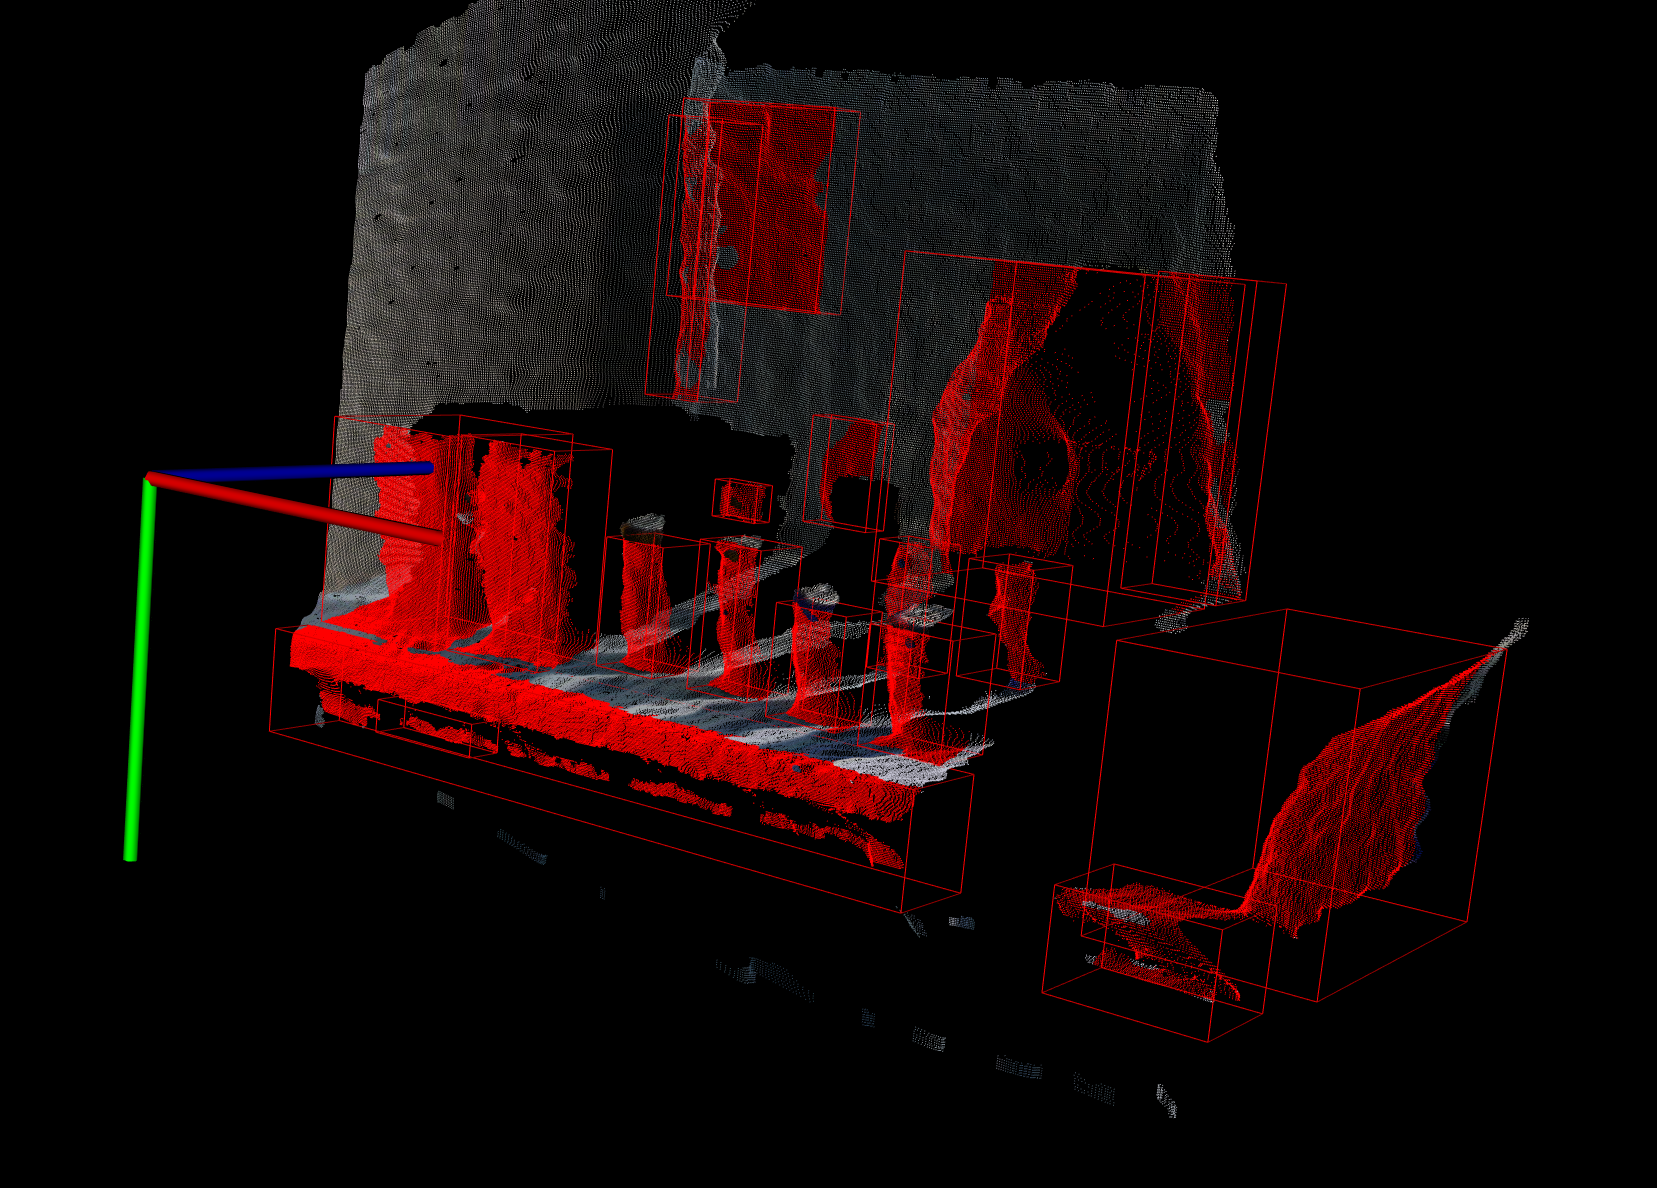
\includegraphics[width=0.9\linewidth]{images/annotated_3Dbboxes_allUnknown.png}
    \caption{Bounding boxes of the clusters obtained after applying the region growing segmentation and leaving only those inside a range of minimum and maximum points inside the cluster. They are marked red since their label is still unknown.}
    \label{fig:annotated_3Dbboxes_allUnknown}
\end{figure}

\subsection{Region growing segmentation and SIFT}
As mentioned earlier, the 3D segmentation deemed to work best is region growing, generating the cluster of figure \ref{fig:annotated_3Dbboxes_allUnknown}. Now, using the camera intrinsic values and the function presented in \ref{eq:project_IntelSDK} implemented in the SDK the 3D bounding boxes are project into 2D bounding boxes, and then passed to a computer vision object recognition algorithm, SIFT specifically. The results are presented in figures \ref{fig:sift_milk_crop}, \ref{fig:sift_pepsi_crop}, \ref{fig:sift_detergent_crop} and \ref{fig:sift_cocacola_crop}. As it can be observed, there are very few matches between the database image and the cropped image. The only object achieving at least 3 pose-consistent matches is the detergent, but 3 is still a low number. Running the experiment multiple times would in some cases render fewer matchings, and hence can not be considered as a consistent method.

\begin{figure}[H]
    \centering
    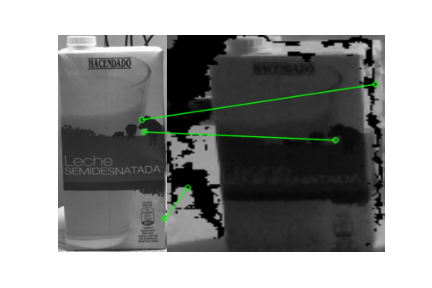
\includegraphics[width=0.7\linewidth]{images/sift_milk_crop.png}
    \caption{\emph{Left}: the database for milk. \emph{Right}: the crop coming from one of the clusters obtained using region growing segmentation. As it can be observed, there's only one good match, and hence not enough to classify it with certainty. artifacts seem to be quite harmful.}
    \label{fig:sift_milk_crop}
\end{figure}

\begin{figure}[H]
    \centering
    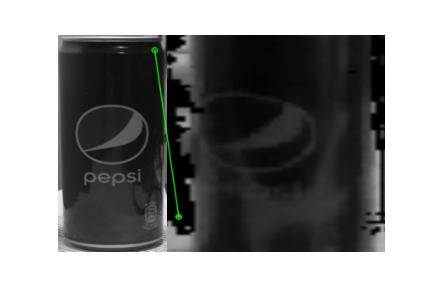
\includegraphics[width=0.7\linewidth]{images/sift_pepsi_crop.png}
    \caption{\emph{Left}: the database for Pepsi. \emph{Right}: the crop coming from one of the clusters obtained using region growing segmentation. As it can be observed, there are no good matches.}
    \label{fig:sift_pepsi_crop}
\end{figure}

\begin{figure}[H]
    \centering
    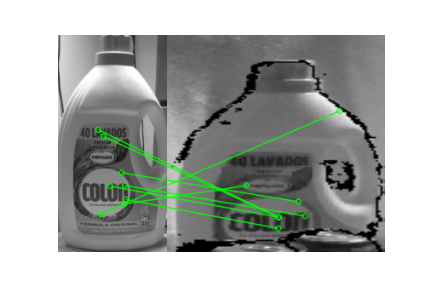
\includegraphics[width=0.7\linewidth]{images/sift_detergent_crop.png}
    \caption{\emph{Left}: the database for Detergent. \emph{Right}: the crop is coming from the clusters obtained using region growing segmentation. As it can be observed, there are 3 good consistent matches, which could be filtered with a RANSAC or Hough voting method.}
    \label{fig:sift_detergent_crop}
\end{figure}

\begin{figure}[H]
    \centering
    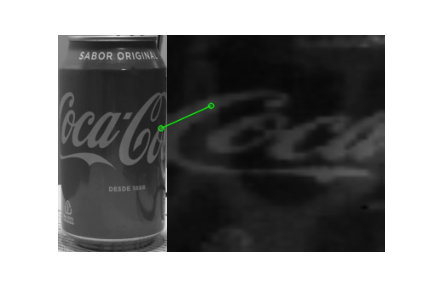
\includegraphics[width=0.7\linewidth]{images/sift_cocacola_crop.png}
    \caption{\emph{Left}: the database for Coca-Cola. \emph{Right}: the crop coming from one of the clusters obtained using region growing segmentation. As it can be observed, there are no good matches.}
    \label{fig:sift_cocacola_crop}
\end{figure}

\subsection{Region growing segmentation and HOG}
Looking at the artifacts present in the RGB image one would suggest that the Histogram of Oriented Gradients is not going to work. And that is indeed the case. Neither the HOG trained with a \emph{k}-NN nor the one with an SVM recognize the crops. Understandably so, looking at the histograms generated from the crops, presented in figures \ref{fig:hog_milk_crop}, \ref{fig:hog_pepsi_crop}, \ref{fig:hog_cocacola_crop} and \ref{fig:hog_detergent_crop}.

\begin{figure}[htbp]
    \centering
    \resizebox{0.7\linewidth}{!}{\import{images/}{hog_milk_crop.pgf}}
    \caption{The histograms of the cells in the images for both the database image and the cropped image. As it can be observed, the artifacts of the cropping clutter too much the crop for it to be of any use.}
    \label{fig:hog_milk_crop}
\end{figure}

\begin{figure}[htbp]
    \centering
    \resizebox{0.7\linewidth}{!}{\import{images/}{hog_pepsi_crop.pgf}}
    \caption{The histograms of the cells in the images for both the database image and the cropped image. The artifacts and the low resolution create vastly different histograms to the ones of the database.}
    \label{fig:hog_pepsi_crop}
\end{figure}

\begin{figure}[htbp]
    \centering
    \resizebox{0.7\linewidth}{!}{\import{images/}{hog_cocacola_crop.pgf}}
    \caption{Same issue as with figure \ref{fig:hog_pepsi_crop}.}
    \label{fig:hog_cocacola_crop}
\end{figure}

\begin{figure}[htbp]
    \centering
    \resizebox{0.7\linewidth}{!}{\import{images/}{hog_detergent_crop.pgf}}
    \caption{Perhaps the detergent provides the most clear HOG descriptors, but still not good enough, since the detector fails. The artifacts in the edges of the object clearly distort it a great deal.}
    \label{fig:hog_detergent_crop}
\end{figure}

\subsection{Region growing segmentation and Template Matching}

\begin{figure}[h]
    \centering
    \resizebox{1\linewidth}{!}{\import{images/}{0pepsiVSmilk_crop_TM.pgf}}
    \caption{Note that the highest peak for the crop belonging to Milk using the Pepsi logo is 0.148. This almost the same value as the one of figure \ref{fig:4pepsi_crop_TM}, where the Pepsi logo is used for a true Pepsi crop. Hence, no classification criterion can be obtained from \texttt{maxVal}.}
    \label{fig:0pepsiVSmilk_crop_TM}
\end{figure}

\begin{figure}[htbp]
    \centering
    \resizebox{1\linewidth}{!}{\import{images/}{4pepsi_crop_TM.pgf}}
    \caption{The Pepsi logo applied to a crop belonging to a Pepsi can. The artifacts, the low resolution and the angle of the image yield an unconclusive peak value. In fact, said \texttt{maxVal} is very close to the one obtained by applying this same Pepsi logo to crops belonging to other classes (see \ref{fig:0pepsiVSmilk_crop_TM}).}
    \label{fig:4pepsi_crop_TM}
\end{figure}

\subsection{Region growing segmentation and a CNN}


\end{document}